\documentclass[11pt, a4paper]{article}

\usepackage{graphicx}
\usepackage[a4paper,top=3cm,bottom=2cm,left=2cm,right=2cm,marginparwidth=1.75cm]{geometry}
\usepackage[english]{babel}
\usepackage[utf8x]{inputenc}
\usepackage{subfig}
\usepackage{float}
\usepackage{amsmath}
\usepackage{amssymb}
\usepackage{mhchem}
\usepackage{hyperref}
\usepackage{tikz}
\usepackage{cancel}

\graphicspath{ {./images} }
\newcommand*{\qed}{\hfill\ensuremath{\quad\square}}%
\newcommand*{\rad}{\ensuremath{\,\text{rad}}}
\newcommand*{\R}{\ensuremath{\mathbb{R}}}
\newcommand*{\C}{\ensuremath{\mathbb{C}}}
\renewcommand*{\Re}{\operatorname{Re}}
\renewcommand*{\Im}{\operatorname{Im}}
\renewcommand*{\epsilon}{\varepsilon}
\renewcommand*{\phi}{\varphi}

\makeatletter
\renewcommand*\env@matrix[1][*\c@MaxMatrixCols c]{%
  \hskip -\arraycolsep
  \let\@ifnextchar\new@ifnextchar
  \array{#1}}
\makeatother

\newtheorem{theorem}{Theorem}

%------------------------------------------------
%Templates for images and figures
% \begin{figure}[h]
%   \centering
%   \subfloat[caption 1]{{
\includegraphics[width=30mm]{images/placeholder.png}}}%
%   \qquad
%   \subfloat[caption 2]{{
\includegraphics[width=30mm]{images/placeholder.png}}}%
%   \caption{Description}
% \end{figure}

% \begin{figure}[h]
%   \centerline{
\includegraphics[width=50mm]{images/placeholder.png}}
%   \caption{Description}
% \end{figure}

%Template for a simple table 
%\begin{table}[h]
%   \caption{Description} %title of the table
%   \centering % centering table
%   \begin{tabular}{l rr} % creating three columns
%     \hline\hline %inserting double-line
%     & & \\ [0.5ex] % Insert half line vertical spacing
%     \hline % inserts single-line
%     & & \\ 
%     & & \\
%     & & \\
%     & & \\
%   \hline % inserts single-line
%   \end{tabular}
%   \label{tab:hresult}
% \end{table}
%-----------------------------------------------

\begin{document}
\setcounter{section}{9}
\setcounter{equation}{0}

\section{Linear Algebra 2 Lecture 10: Quadratic forms (29/05/2020)}

\subsection{Definition of a quadratic form}
A function $Q(\vec{x}): \R^n \to \R$ is called a quadratic form if it can be written in the form $Q(\vec{x}) = \vec{x}^TA\vec{x}$, where $A$ is a symmetric $n \times n$ matrix. The simplest example of this is the situation where $A=I_n$:
\begin{align}
  Q(\vec{x}) = \vec{x}^TI\vec{x} = \vec{x}^T\vec{x} &= ||\vec{x}||^2\\
  &= x_1 + x_2 + \cdots + x_n
\end{align}
Every quadratic form can be expressed as:
\begin{equation}
  Q(\vec{x}) = \sum_{i=1}^n \sum_{j=1}^n a_{ij}x_ix_k
\end{equation}
There exists a symmetric $n \times n$ matrix such that:
\begin{equation}
  Q(\vec{x}) = \vec{x}^T A \vec{x}
\end{equation}
for every vector $\vec{x} \in \R^n$.


\subsection{Finding a quadratic form for a given matrix $A$}
let $A = \begin{bmatrix} 3 & -2\\ -2 & 7\\ \end{bmatrix}$ and $\vec{x} = \begin{bmatrix} x_1 \\ x_2 \end{bmatrix}$. Then:
\begin{align*}
  Q(\vec{x}) &= \vec{x}^T A \vec{x}\\
  &= \begin{bmatrix} x_1 & x_2\\ \end{bmatrix} \begin{bmatrix} 3 & -2\\ -2 & 7\\ \end{bmatrix} \begin{bmatrix} x_1 \\ x_2 \\ \end{bmatrix}\\
  &= \begin{bmatrix} x_1 & x_2 \\ \end{bmatrix} \begin{bmatrix} 3x_1-2x_2\\ -2x_1 + 7x_2 \\ \end{bmatrix}\\
  &= x_1(3x_1-2x_2) + x_2(-2x_1 + 7x_2)\\
  &= 3x_1^2 + 7x_2^2 - 4x_1x_2
\end{align*}
Where the term $4x_1x_2$ is referred to as the cross-product term. There are methods such as a change of variables to get rid of this cross-product term whcih will be discussed later.


\subsection{Finding the matrix $A$ for a given quadratic form}
Let $Q(\vec{x}) = 5x_1^2 + 3x_2^2 + 2x_3^2 - 2x_1x_2 + 8x_2x_3 = \vec{x}^TA\vec{x}$.
The vector $\vec{x}$ has $3$ entries, and the matrix $A$ is symmetric. Thus $A$ should be a $3 \times 3$ matrix. It's main entries will be the squared terms of $Q(\vec{x})$.\\
Since $A$ is a symmetric matrix the cross-product terms need to be split evenly between $a_{ij}$ and $a_{ji}$. Thus $a_{12}$ and $a_{21}$ should be $\frac{1}{2}\cdot -2 = -1$, $a_{23}$ and $a_{32}$ should be $\frac{1}{2}\cdot 4 = 2$ and $a_{13}$ and $a_{31}$ should both be $0$. This leaves us with the following matrix $A$:
\begin{equation*}
  A = 
  \begin{bmatrix}
    5 & -1 & 0\\
    -1 & 3 & 4\\
    0 & 4 & 2\\  
  \end{bmatrix}
\end{equation*}


\subsection{The principal axes theorem}
Let a quadratic form $Q(\vec{x})$ be given for some symmetric $n \times n $ matrix $A$. $A$ being symmetric guarantees that there exists an orthogonal matrix $P$ such that $\vec{x} = P\vec{y}$. This transforms the quadratic form $Q(\vec{x})$ to a different quadratic form denoted as $\bar{Q}(\vec{y})$. The diagonal matrix $D$ can be expressed as $D = P^TAP$, thus:
\begin{equation}
  \bar{Q}(\vec{y}) = \vec{y}^T D \vec{y}
\end{equation}
Since $D$ is a diagonal matrix we can know for certain that the quadratic form $\bar{Q}(\vec{y})$ will not have any cross-product terms. We also know that $D$ was constructed to have the eigenvalues of $A$ as it's main entries. The expression for $\bar{Q}(\vec{y})$ then reduces to:
\begin{equation}
  \bar{Q}(\vec{y}) = \lambda_1 y_1^2 + \lambda_2 y_2^2 + \cdots + \lambda_n y_n^2
\end{equation}
The principal axes of the quadratic form $Q$ are the lines generated by the columns of $P$. It can be thought of as the geometrical counterpart of the spectral theorem. It has application in dynamics such as when computing the moment of inertia tensor.


\subsection{Algorithm for removing cross-product terms}
Let $Q(\vec{x})$ be a quadratic form with symmetric matrix $A$:
\begin{enumerate}
  \item orthogonal diagonalization: $A = PDP^T$. Define a basis $\mathcal{B} = \{ \vec{u}_1, \cdots \vec{u}_n\}$ to be orthonormal and consisting of the columns of $P$.
  \item Define a new variable $\vec{y} = [\vec{x}]_\mathcal{B} = P^T\vec{x}$. Note that the matrix $P$ is orthogonal and thus $P^{-1} = P^T$. This implies $\vec{x} = P\vec{y}$
  \item Then: $Q(\vec{x}) = \vec{x}^T A \vec{x} = \vec{y}^T D \vec{y}$.
\end{enumerate}


\subsection{Classification of quadratic forms}
The quadratic form $Q(\vec{x})$ is:
\begin{itemize}
  \item positive semidefinite if $Q(\vec{x}) \geq 0$ for all $\vec{x}$. This happens when all $\lambda \geq 0$
  \item positive definite if $Q(\vec{x}) > 0$ for all $\vec{x} \neq 0$. This happens when all $\lambda > 0$
  \item negative semidefinite if $Q(\vec{x}) \leq 0$ for all $\vec{x}$. This happens when all $\lambda \leq 0$
  \item negative definite if $Q(\vec{x}) < 0$ for all $\vec{x} \neq 0$. This happens when all $\lambda < 0$.
  \item indefinite if $Q(\vec{x})$ assumes both positive and negative values. This happens when $\lambda$ has both positive and negative values. 
\end{itemize}
\begin{figure}[h]
  \centering
  \subfloat[Positive definite]{{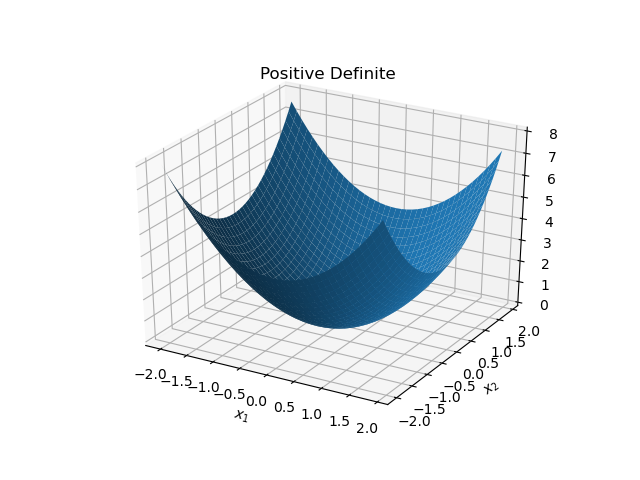
\includegraphics[width=50mm]{images/pd_plot.png}}}%
  \qquad
  \subfloat[Negative definite]{{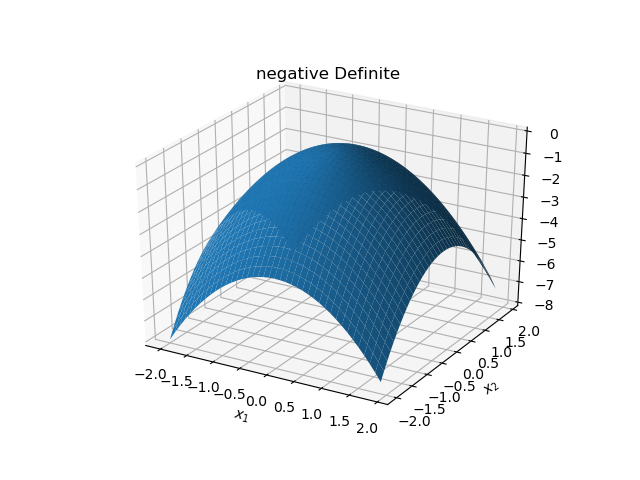
\includegraphics[width=50mm]{images/nd_plot.png}}}%
  \qquad
  \subfloat[Indefinite]{{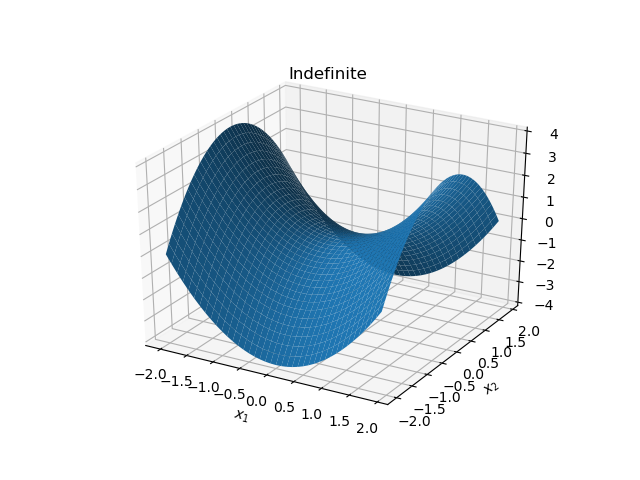
\includegraphics[width=50mm]{images/id_plot.png}}}%
  \caption{Surface plots of the classifications of quadratic forms using matplotlib and Python}
\end{figure}



\end{document}